% !TEX root = ./main.tex
%%%%%%%%%%%%%%%%%%%%%%%%%%%%%%%%%%%%%%%%%%%%%%%%%%%%%%%%%%%%%%%%%%%%%%%%%%%%%%%%%%%%%%%%%%
% Dans cette section, indiquez et décrivez tous les Invariants nécessaires.              %
%                                                                                        %
% Pour chaque SP nécessitant un Invariant (une sous-section/SP):                         %
% - Donnez l'Invariant Graphique                                                         %
% - Donnez l'Invariant Formel correspondant à l'Invariant Graphique                      %
% Pensez à utiliser les notations définies précédemment.                                 %
%%%%%%%%%%%%%%%%%%%%%%%%%%%%%%%%%%%%%%%%%%%%%%%%%%%%%%%%%%%%%%%%%%%%%%%%%%%%%%%%%%%%%%%%%%
\section{Invariants}\label{invariants}
%%%%%%%%%%%%%%%%%%%%

\subsection{Invariant du temps total}

\begin{figure}[h]
    \centering
    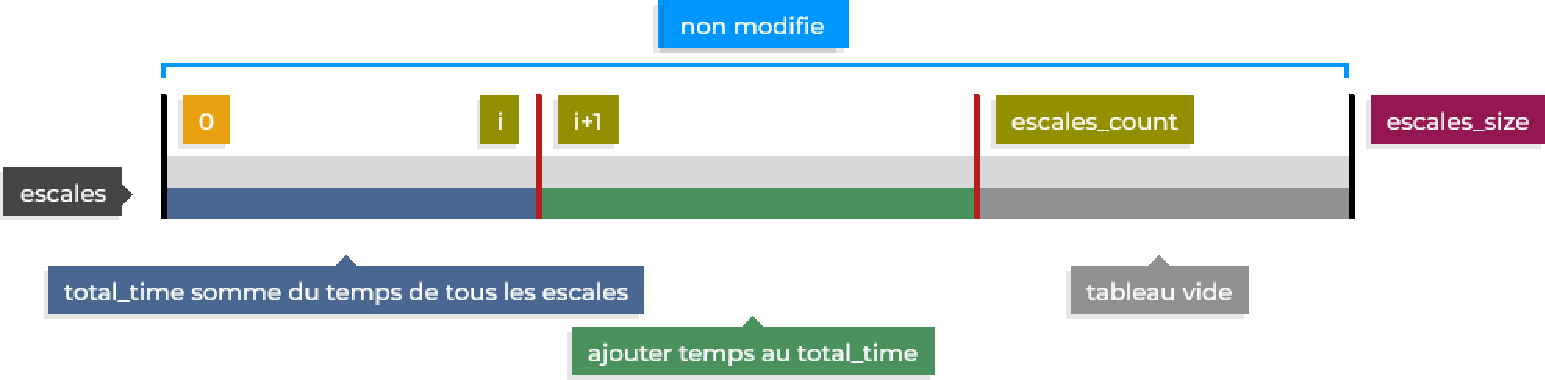
\includegraphics[width=1\textwidth]{invariant_time.pdf}
    \caption{Invariant graphique}
\end{figure}

\textbf{Invariant formel:} \\
    $escale = escale_0$ \\
    $\land$ \\
    $0 < i < escale\_count$ \\
    $\land$ \\
    $total\_time = \sum_{i=0}^{escale\_count-1} \texttt{escale\_get\_best\_time}(escales[i])$
